%!TEX root = ../main.tex

\section{Experimental apparatus}

The NREL 2FBR reactor system thermochemically converts biomass feedstock at fast pyrolysis conditions. The system is comprised of two bubbling fluidized bed (BFB) reactors where the first reactor is for biomass fast pyrolysis and the second reactor is for vapor phase upgrading. An overview of the NREL 2FBR system is shown in Figure \ref{fig:nrel-system}, components of the pyrolysis reactor are detailed in Figure \ref{fig:pyrolyzer-components}, while dimensions and typical operating conditions of the pyrolysis unit are given in Figure \ref{fig:pyrolyzer-dims-flows}. Sand is used as the fluidization medium in the pyrolyzer. Biomass particles are fed to the reactor via a screw auger and nitrogen is used as the fluidization/carrier gas. More information about the NREL 2FBR biomass pyrolysis system is available elsewhere \cite{Howe-2015, Trendewicz-2015}. Yields from the BFB pyrolysis reactor are compared to model results discussed later in this paper.

\begin{figure}[H]
    \centering
    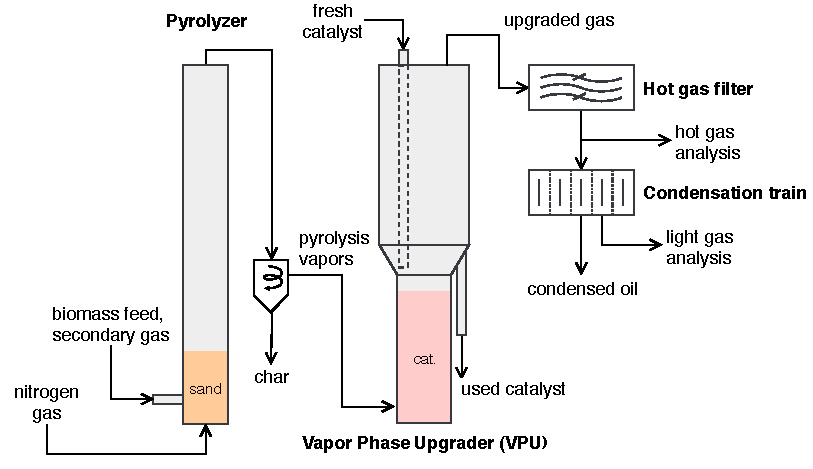
\includegraphics[width=0.8\textwidth]{system.pdf}
    \caption{Overview of the NREL 2FBR system. Biomass fast pyrolysis occurs in the pyrolyzer (left) and gaseous products are catalytically upgraded in the vapor phase upgrader (right).}
    \label{fig:nrel-system}
\end{figure}

\begin{figure}[H]
    \centering
    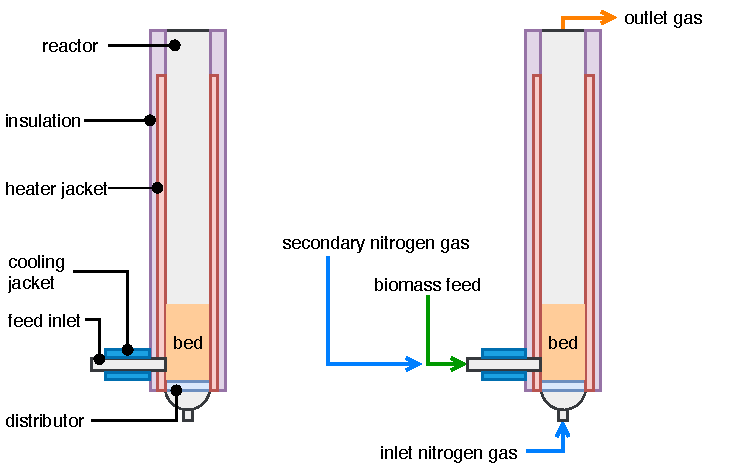
\includegraphics[width=0.8\textwidth]{pyrolyzer-components.pdf}
    \caption{Components of the BFB biomass pyrolysis reactor referred to as the ``pyrolyzer'' in the NREL 2FBR system.}
    \label{fig:pyrolyzer-components}
\end{figure}

\begin{figure}[H]
    \centering
    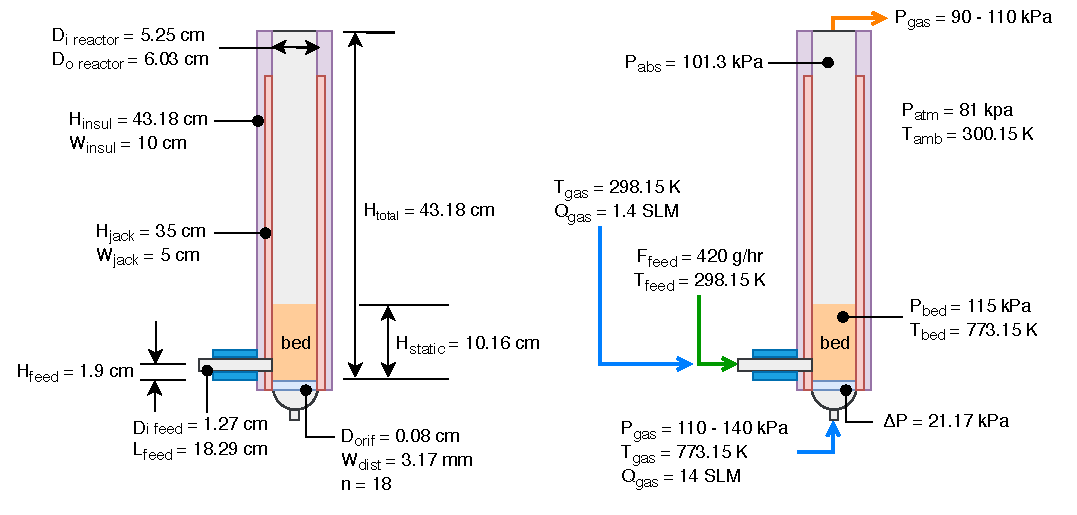
\includegraphics[width=\textwidth]{pyrolyzer-dims-flows.pdf}
    \caption{Dimensions and typical fast pyrolysis operating conditions for the BFB biomass pyrolysis reactor in the NREL 2FBR system.}
    \label{fig:pyrolyzer-dims-flows}
\end{figure}
